% *******************************************************************************
% * Copyright (c) 2007 by Elexis
% * All rights reserved. This document and the accompanying materials
% * are made available under the terms of the Eclipse Public License v1.0
% * which accompanies this distribution, and is available at
% * http://www.eclipse.org/legal/epl-v10.html
% *
% * Contributors:
% *    G. Weirich - initial implementation
% *
% *  $Id$
% *******************************************************************************
%
% !Mode:: "TeX:UTF-8" (encoding info for WinEdt)


\section{Configuration de base}
Pour seulement tester le logiciel vous n'avez pas besoin de lire ce chapitre. L'installateur standard d'Elexis contient une base de données version démo qui devait être suffisant pour les tests.

Pour la véritable utilisation du logiciel par contre on ne s'échappe pas à une configuration assez laborieuse. Vous devez pourtant introduire tous les données qui sont spécifiques pour votre cabinet médical.

\subsection{Remarque préliminaire}
Si vous pensez accomplir ce travail de configuration vous-même, il faudra réserver suffisamment de temps (plusieurs heures à une journée entière). Nous vous conseillons d'imprimer les instructions et de suivre ce chapitre étape par étape. Si vous n'êtes pas sûr comment configurer Elexis, nous vous conseillons vivement d'engager un prestataire de service compétent car les fautes commises lors de cette configuration pourraient entraver plus tard un travail correct.

\subsection{Ce dont vous avez besoin}
Avant de commencer la configuration vous devez collectionner les programmes et données suivants :
\begin{itemize}
  \item Noms, Noms d'utilisateur et mots de passe pour tous qui devaient pouvoir utiliser Elexis
  \item Noms, Numéros du Concordat , Numéros EAN, Coordonnées bancaires ou pour le compte de chèque postal, numéros de participant BVR de tous les mandants.
  \item Une conception de vos en-têtes pour lettres, ordonnances, certificats.
  \item Une liste des examens de laboratoire effectués dans votre laboratoire du cabinet.
  \item Liste des médicaments, CIM-10, Tarmed , Liste des analyses, MiGel dans la mesure où vous en avez besoin.
  \item Les numéros EAN des assurances maladies et accidents
\end{itemize}
\subsection{Premier pas : Créer un lien avec la base de données}
Si vous démarrez Elexis pour la première fois, une base de données HSQL locale sera crée. Pour travailler sur ce poste isolé il n'y a aucune restriction pour son utilisation. Si vous souhaitez par contre travailler dans un environement à usagers multiples, il faut que Elexis soit lié à une base de donnée sur un serveur centrale au lieu d'être liée seulement à la base de données locale. Dans ce qui suit on présume que le serveur a déjà été installé selon la proposition faite sur
\href{http://www.elexis.ch/jp/index.php?option=content&task=view&id=72}{Datenbank}
Veuillez démarrer Elexis et sélectionnez dans le menu principal\textit{Fichier-Lien} . 
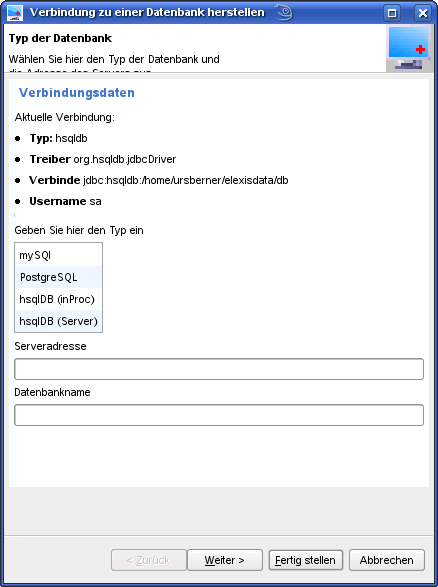
\includegraphics[width=3.5in]{images/verb1.png}
% verb1.png: 438x587 pixel, 72dpi, 15.45x20.71 cm, bb=0 0 438 587

Veuillez inroduire le type de banque de données, l'adresse TCP/IP du serveur et le nom de la banque de données et cliquez sur \textit{next}

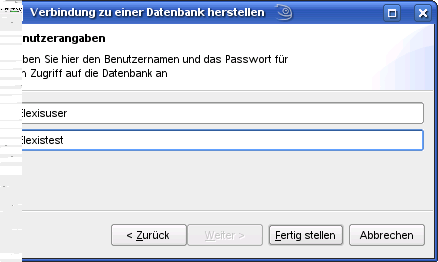
\includegraphics[width=3.5in]{images/verb2.png}
% verb2.png: 438x262 pixel, 72dpi, 15.45x9.24 cm, bb=0 0 438 262

Finalement veuillez introduire le nom de l'utilisateur et le mot de passe comme vous l'avez introduit lors de l'installation de la banque de données et cliquez sur \textit{finish}.
Si votre installation est en ordre votre ordinateur devrait être capable de accéder au serveur.

\subsection{\index{mandant}Deuxième pas: installer les mandants et les utilisateurs}
Veuillez ouvrir la perspective \textit{contacts},

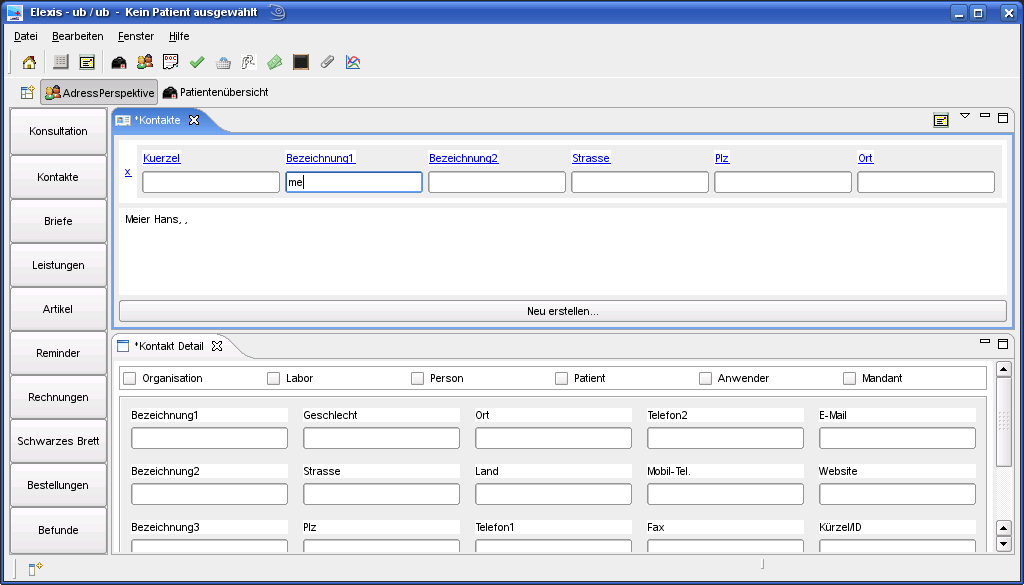
\includegraphics[width=4.5in]{images/grundkonfkonta.png}
% grundkonfkonta.png: 1024x585 pixel, 72dpi, 36.12x20.64 cm, bb=0 0 1024 585
\begin{itemize}
 \item Veuillez introduire sous \textit{désignation1} le nom du nouveau mandant ou d'un nouvel utilisateur  et cliquez sur \textit{constituer}
 \item Cherchez ensuite l'inscription que vous venez de fair dans la liste supérieure. Séléctionnez la et veuillez la compléter dans la partie inférieure. Comme d'habitude dans Elexis vous n'êtes pas forcé de remplir tous les champs.
 \textit{Désignez} le contact que vous venez de créer comme \textit{mandant} ou \textit{utilisateur} (Un mandant est toujours aussi un utilisateur et les deux sont toujours aussi des  \textit{personnes}
 \item WAprès avoir fini l'introduction de tous les mandants et utilisateurs veuillez choisir Fichier - Paramètres et ensuite l'onglet \textit{contrôle d'accès - mandants}
\end{itemize}

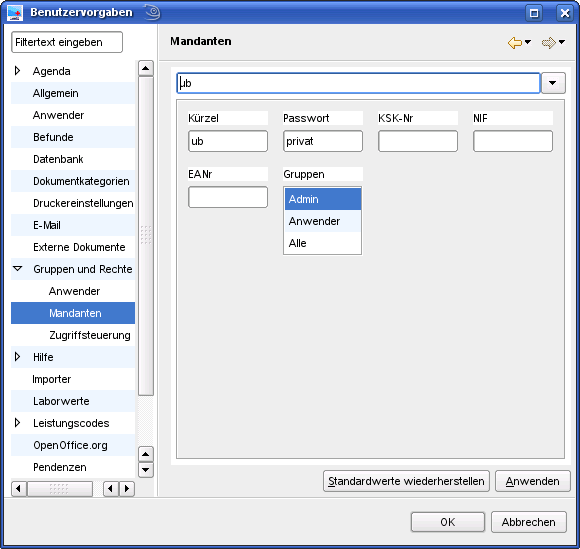
\includegraphics[width=4in]{images/grundkonfmand.png}
% grundkonfmand.png: 580x549 pixel, 72dpi, 20.46x19.37 cm, bb=0 0 580 549
\begin{itemize}
 \item Veuillez introduire là les indications pour les mandants installés. Veuillez introduire comme\textit{sigle} le nom du mandant et comme mot de passe le mot de passe défini. Le reste des données à introduire dépendent du type du mandant.
 \item Allez ensuite vers la section contrôle d'accès - utilisateurs.
\end{itemize}

Veuillez y introduire pour tous \index{utilisateurs}les utilisateurs déjà définis les données correspondantes. N'oubliez pas d'assigner à tous les utilisateurs un mandant standard existant. (\textit{pour mandant}). Un mandant standard doit aussi être assigné pour pour des mandants déjà introduits (que vous trouvez dans les paramètres des utilisateurs, car les mandants sont aussi des utilisateurs) mais normalement les mandants sont assignés à eux-mêmes. L'assignation au mandant définit au nom de qui et pour qui l'utilisateur travaille normalement. Ceci peut changer à tout moment pendant le travail journalier (sous \textsc{fichier - mandant}...), mais lors du login il faut toujours choisir d'abord un mandant standard.

\subsection{Troisième pas: introduire les paramètres du laboratoire}
Veuillez tout d'abord ouvrir de nouveau la\textit{View - contacts}. Introduisez là votre propre laboratoire et les laboratoires externes avec lesquels vous collaborez.
Veuillez les marquer comme \textit{laboratoire}

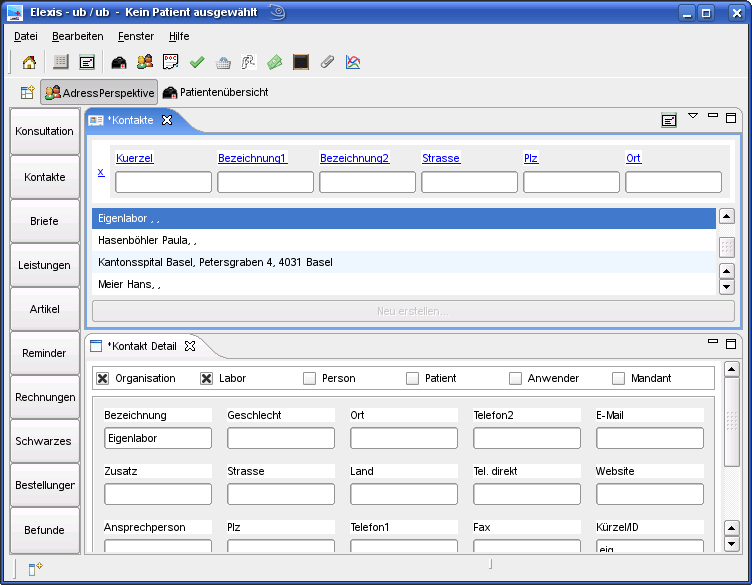
\includegraphics[width=4in]{images/grundkonfmand1.png}
% grundkonfmand1.png: 752x585 pixel, 72dpi, 26.53x20.64 cm, bb=0 0 752 585
\subsection{Quatrième pas: configurer le logiciel pour traitement de texte}

Jusqu'alors Elexis ne travaille qu'avec OpenOffice, raison pour laquelle nous expliquons ici que la configuration avec  OpenOffice.
Séléctionnez dans Elexis \textsc{Fichier-Paramètres-traitement de texte}

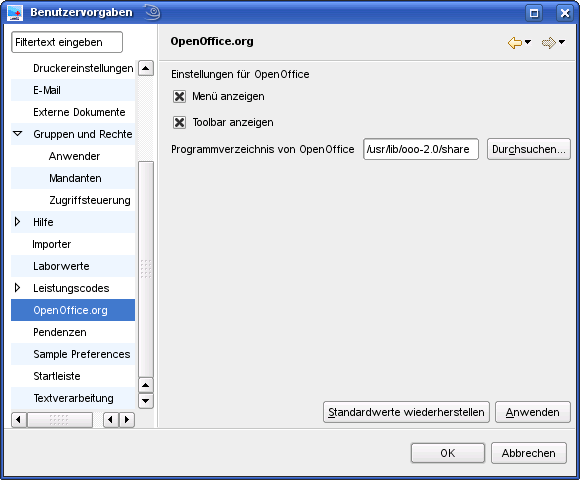
\includegraphics[width=3.5in]{images/grundkonfmand2.png}
% grundkonfmand2.png: 580x480 pixel, 72dpi, 20.46x16.93 cm, bb=0 0 580 480

\begin{itemize}
 \item Cherchez le chemin d'accès du\textit{program} sous-répertoire de l'installation de OpenOffice. Sous Windows ceci se trouvera normalement sous c:/programme/OpenOffice.org 2.0/program  respectivement à l'endroit où vous avez installé OpenOffice.
 \item Choisissez \textit{Apply},fermez ensuite la configuration et redémarrez Elexis.
 \item Si vous séléctionnez maintenant par exemple la perspective lettres, la fenêtre de OpenOffice devait s'ouvrir à l'intérieur de la fenêtre de Elexis. (Lors du premier accès ceci peut durer assez longtemps càd environs 30 secondes)
\end{itemize}

\subsubsection{Cinquième pas: \index{modèles!formulaires}créer modèles formulaires}
Pour certains formulaires Elexis cherche un modèle prédéfini avec un nom fixe. Ceci définit l'apparence spécifique de ces formulaires pour vos applications. Des variables douvent être introduits aux endroits prédéfinis.

Pour créer un modèle vous procédez de préférence de façon suivante : Ecrivez votre modèle tout simplement dans votre logiciel de traitement de texte et sauvegardez-le comme document texte. Séléctionnez depuis Elexis la perspective \textit{lettres} et choisissez le


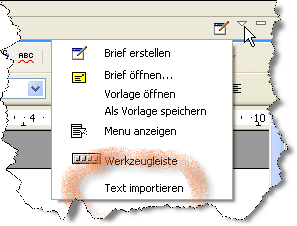
\includegraphics[width=2.5in]{images/import.png}
% import.png: 297x226 pixel, 96dpi, 7.86x5.98 cm, bb=0 0 223 169

menuView à droite.

Vous y choisissez \textit{importer texte} uet cherchez votre modèle que vous venez d'écrire. Par ceci vous importez le document dans Elexis. A ce stade vous pouvez encore faire des adaptations. Ensuite vous séléctionnez de nouveau le menu View à droite et choisissez cette fois-ci  \textit{sauvegarder comme modèle}.

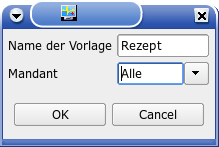
\includegraphics[width=2.5in]{images/rezept1.png}
% rezept1.png: 219x147 pixel, 72dpi, 7.73x5.19 cm, bb=0 0 219 147

Pour le\textit{nom du modèle} vous devez introduire en bas dans la liste des modèles standard le nom choisi. (Pour vos propres modèles vous pouvez introduire un nom quelconque. Sous \textit{mandant} vous pouvez assigner le mandant pour lequel vous avez crée ce modèle (vous pouvez aussi chosir qu'il est pour tous les mandants).

Figurant ci dessous une liste des modèles standards :

\begin{itemize}
\item Ordonnance: \index{modèle!ordonnance} Vous nécessitez pour ceci un modèle avec le nom \textit{ordonnance}. Il peut se voir par exemple de cette manière :
 \end{itemize}
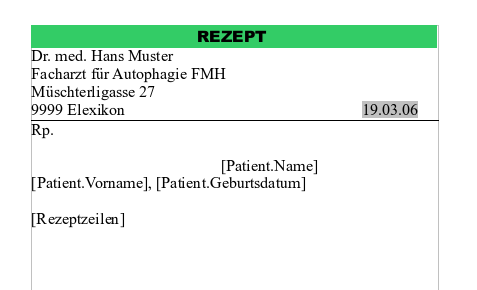
\includegraphics[width=4in]{images/rezept.png}
% rezept.png: 477x290 pixel, 72dpi, 16.83x10.23 cm, bb=0 0 477 290

A l'emplacement où se trouve [lignes de l'ordonnance] vous introduisez plus tard les médicaments. Cette variable est par conséquent indispensable. Tous les autres éléments du modèle \textit{ordonnance} sont  facultatifs.

\begin{itemize}
 \item \textit{Certificat médical}: Un modèle pour les certificats médicaux. On peut introduire comme variable [incap.raison], [incap.de], [incap.à], [incap.pourcentage] et toutes les variables standards. Toutes sont facultatives.

 \item \textit{feuille labo}: Pour la mise en page des résultats du laboratoire. Les différentes valeurs du laboratoire sont introduites à la place de la variable [valeurs du laboratoire]. Cette variable est indispensable d'autres peuvent être introduites selon besoin.
\end{itemize}

\subsubsection{Sixième pas: Introduire des banques de données externes}

Elexis peut importer une série des données de base depuis des soureces externes. Veuillez être attentifs sur le fait que ces sources pourrait être soumises à un Copyright. En cas de doute il est recommandable de s'informer auprès de l'organisation qui publie la source.

\begin{description}
 \item[Tarmed] \index{base de données!Tarmed}Depuis le site \href{www.tarmedsuisse.ch}{Tarmed} peut être téléchargé comme base de données Microsoft-Access. Veuillez l'intégrer dans un ordinateur avec Windows en tant que DNS (système de noms de domaine). Choisissez dans Elexis sous perspective \textit{codes} , séléctionnez là l'onglet\textit{Tarmed}  et ouvrez à droite le menuView. 
 Séléctionnez  \textit{import}  et introduisez le Tarmed-DSN que vous venez de configurer. Dépendant de la vitesse de l'ordinateur l'importation de toute la base de données prendra entre une et 5 minutes. Vous trouvez ici ??????? des instructions détaillées.
 \item[CIM-10] Au site ???????????
 \href{http://www.dimdi.de/dynamic/de/klassi/downloadcenter/icd-10-who/version2006/systematik/}{DIMDI} vous pouvez télécharger le catalogue CIM_10 de l'OMS en format XYYYYY. Vous avez besoin de \textit{ICD-10-WHO-Systematik EDV-Fassung ASCII} und die \textit{ICD-10-WHO-2006 Systematik Metadaten ASCII}. Ouvrez les deux Zip dans le même répertoire. VOus pouvez ignorer l'avertissement que vous allez écraser un fichier. Ensuite vous allez dans Elexis sur la \textit{perspektive-codes} et là sur l'onglet \textit{ICD-10}et choisissez de nouveau \textit{import} dans le menu- view.
 Dans la boîte de dialogue suivant veuillez indiquer le répertoire dans lequel vous avez installé le Code CIM-10.  u
 \item[Médicament et  Medicals] \indexname{données de base!médicaments}Ces deux groupes sont constitués de la même base de données. Vous nécessitez la liste\textit{transfer.dat}, que vous pouvez acheter par exemple de\textit{www.e-mediat.ch} en forme d'abonnement.
 Sélectionnez la perspective \textit{codes} , ensuite cliquez sur l'onglet Medicals réspectivement médicaments et là de nouveau dans le menu-view l'option import et introduisez le chemin d'accès pour le fichier transfer.dat.
\textit{Remarque: Depuis peu existe une liste des spécialités de l'OFSP en forme d'un fichier Excel. Le module d'importation pour ce format est en voie de développement. Ceci permettra de pouvoir se passer du fichier transfer.dat payant. }
 \item[liste des analyses et LiMA] \index{base de données!liste des analyses et LiMA}Ceux-ci sont publiés par l'OFSP mais malheureusement, pour des raisons inintelligibles qu'en format pdf. Ceci provoque qu'on doit faire un pas de conversion pour extraire de ce fichier pdf les données utiles, chose qui comporte toujours un certain risque de faire des fautes. Pour ce procédé vous nécessitez un logiciel par exemple sous Windows TextFromPDF, ou sous Linux xpdf. A l'aide de ce programme il faut créer une version-plaintexte de la liste des analyses. Ensuite vous ouvrez Elexis dans la perspective  \textit{codes}  et choisissez là l'onglet \textit{analyses} réspectivement LiMA. Il faudra de nouveau choisir l'  \textit{import} dans le menu-view et introduire le chemin d'accès au fichier qui contient les données converties.
 \end{description}

\subsubsection{Septième pas: Transférer réspectivement introduire les données des patients}
Maintenant vous avez achevé les préparatifs et pouvez commencer à introduire les propres données que vous nécessitez pour travailler. Pour ceci veuillez procéder pour tous les patients de façon uniforme comme c'est décrit dans la partie 'visite guidée'.


